% !TeX spellcheck = en_US

% We need layers to draw the block diagram
\usetikzlibrary{calc,positioning}
\usetikzlibrary{arrows.meta}

% Define a few styles and constants
\tikzstyle{entry}=[draw, fill=green!20, minimum height=2.5em]
\tikzstyle{ann} = [above, text width=5em]
\tikzstyle{framework} = [entry, text width=30em, fill=white, 
minimum height=20em, rounded corners]
\tikzstyle{lang} = [entry, text width=9em, shading = axis,rectangle, left color=blue!10!white, right color=blue!30!white,shading angle=135, anchor=north,
minimum height=3em, rounded corners]
\tikzstyle{control} = [entry, text width=11em, shading = axis,rectangle, left color=blue!10!white, right color=blue!30!white,shading angle=135, anchor=north,
minimum height=12em, rounded corners]
\tikzstyle{core} = [entry, text width=14em, shading = axis,rectangle, left color=blue!10!white, right color=blue!30!white,shading angle=135, anchor=north,
minimum height=3em, rounded corners]
\tikzstyle{ia} = [entry, text width=9em, shading = axis,rectangle, left color=blue!10!white, right color=blue!30!white,shading angle=135, anchor=north,
minimum height=4em, rounded corners]
\tikzstyle{service} = [entry, text width=9em, shading = axis,rectangle, left color=blue!10!white, right color=blue!30!white,shading angle=135, anchor=north,
minimum height=4em, rounded corners]
\tikzstyle{plan} = [entry, text width=9em, shading = axis,rectangle, left color=blue!10!white, right color=blue!30!white,shading angle=135, anchor=north,
minimum height=4em, rounded corners]
\tikzstyle{item} = [entry, text width=8em, shading = axis,rectangle, left color=blue!20!white, right color=blue!40!white,shading angle=135, anchor=north,
minimum height=1em, rounded corners]
\def\blockdist{2.3}
\def\edgedist{2.5}

\begin{figure}
	\centering
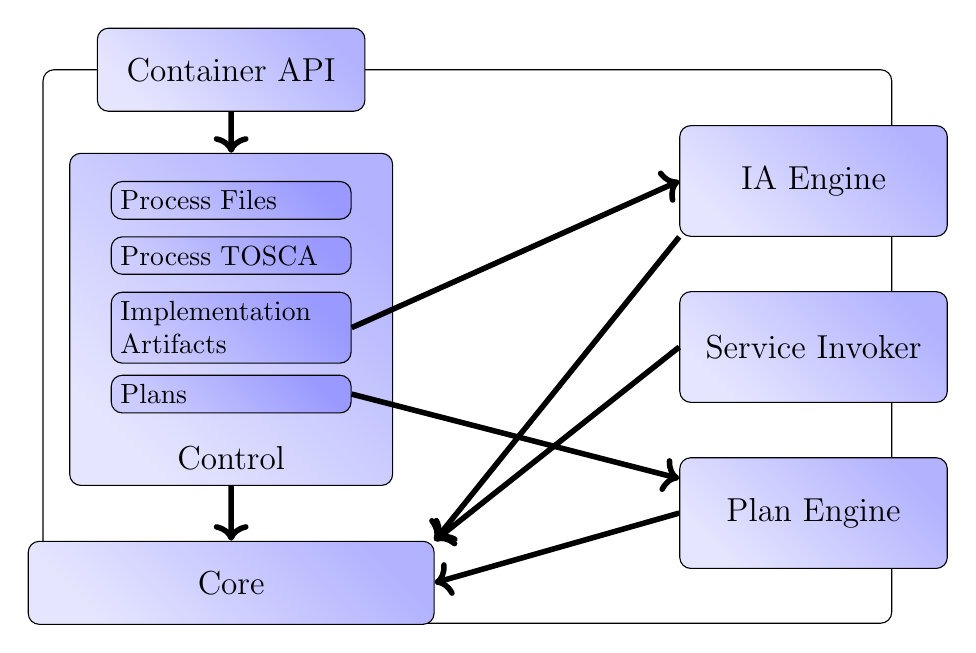
\begin{tikzpicture}
\node (rr) [framework] {};


\node (lang1) [xshift=-30mm, yshift=+1.5em] at ( rr.north) [lang] {};
\node at (lang1) {\large Container API};

\node (control) [xshift=-30mm, yshift=+7em] at ( rr) [control] {};
\node [yshift=+1em] at (control.south) {\large Control};

\node [xshift=-0mm, yshift=+5em] at ( control) [item] {Process Files};
\node [xshift=-0mm, yshift=+3em] at ( control) [item] {Process TOSCA};
\node (impl)[xshift=-0mm, yshift=+1em] at ( control) [item] {Implementation Artifacts};
\node (plans)[xshift=-0mm, yshift=+-2em] at ( control) [item] {Plans};

\node (core) [xshift=-30mm, yshift=+3em] at ( rr.south) [core] {};
\node at (core) {\large Core};

\node (ia) [xshift=-10mm, yshift=+8em] at ( rr.east) [ia] {};
\node at (ia) {\large IA Engine};

\node (service) [xshift=-10mm, yshift=+2em] at ( rr.east) [service] {};
\node at (service) {\large Service Invoker};

\node (plan) [xshift=-10mm, yshift=-4em] at ( rr.east) [plan] {};
\node at (plan) {\large Plan Engine};

\draw [->,scale=5,line width=2pt] (lang1) -- (control);
\draw [->,scale=5,line width=2pt] (control) -- (core);
\draw [->,scale=5,line width=2pt] (plan.west) -- (core.east);
\draw [->,scale=5,line width=2pt] (service.west) -- (core.north east);
\draw [->,scale=5,line width=2pt] (ia.south west) -- (core.north east);
\draw [->,scale=5,line width=2pt] (impl.east) -- (ia.west);
\draw [->,scale=5,line width=2pt] (plans.east) -- (plan);
\end{tikzpicture} 
\caption{OpenTOSCA runtime environment control flow} 	\label{fig:opencontainer}
\end{figure}